\chapter{Results and Discussion}
\label{chap:results}

\section{Simulation Environment and Setup}
\label{sec:simulation_setup}
\subsection{Static Known-Geometry Benchmark}
The benchmark contains 100 static environments: 60 for training, 20 for validation and 20 for testing. Arenas measure $10\times10\times6.5$\,m, with obstacle occupancy from 1\% to 12.5\% and geometry known to every method. Each start--goal pair has a verified three-dimensional A* reference and a budget based on twice its length.

Commands are issued at 20\,Hz, with each velocity component bounded by 1.5\,m/s. The nominal barrier uses $\alpha=4$ and a 0.28\,m offset: a 0.18\,m vehicle envelope plus a 0.10\,m clearance buffer. An episode succeeds on reaching the 0.40\,m goal region. Its collision event is an overlap of the 0.18\,m evaluation envelope with an obstacle or wall; the collision check takes precedence over goal attainment.

\subsection{Physics-Based Navigation Extension}
The practical extension uses Isaac Sim and MuJoCo, with pillar obstacles and local mapping from simulated LiDAR observations containing noise and missing returns. A planned A* route is smoothed with a B-spline. The three comparison scenarios contain 72 static obstacles together with 12, 20 or 40 dynamic obstacles. The scene views and the NavRL comparison appear in Section~\ref{chap:sim2real}; they complement the known-geometry disturbance benchmark.

\clearpage
\section{Performance Metrics}
\label{sec:performance_metrics}

\subsection{Safety and Episode Outcomes}

We evaluate safe mission completion and tracking accuracy under disturbance using the following performance metrics.

Consider $N$ evaluation episodes. We assign each episode one terminal outcome: success, collision or timeout. Success means reaching the goal within the prescribed tolerance and time limit without collision. A collision ends the episode; an episode that reaches neither a successful goal nor a collision before the time limit is a timeout. If goal attainment and collision occur at the same step, collision takes precedence.

Let $N_{\mathrm{S}}$, $N_{\mathrm{C}}$ and $N_{\mathrm{T}}$ denote the corresponding counts. The success rate (SR), collision rate (CR) and timeout rate (TR) are
\begin{equation}
 \mathrm{SR}=\frac{N_{\mathrm{S}}}{N},\qquad
 \mathrm{CR}=\frac{N_{\mathrm{C}}}{N},\qquad
 \mathrm{TR}=\frac{N_{\mathrm{T}}}{N}.
 \label{eq:episode_rates}
\end{equation}
These fractions are reported as percentages. Under this three-outcome convention, $\mathrm{SR}+\mathrm{CR}+\mathrm{TR}=1$.

\begin{table}[H]
\centering
\caption{Interpretation of the episode-outcome metrics.}
\label{tab:episode_metrics}
\renewcommand{\arraystretch}{1.35}
\begin{tabularx}{\linewidth}{@{}lYc@{}}
\toprule
\textbf{Metric} & \textbf{What it measures} & \textbf{Desired}\\
\midrule
\textcolor{teal}{\textbf{SR}} & Safe mission completion & Higher\\
\textcolor{navy}{\textbf{CR}} & Episodes ending in collision & Lower\\
\textbf{TR} & Episodes exhausting their time budget & Lower\\
\bottomrule
\end{tabularx}
\end{table}

SR measures safe mission completion, CR isolates collision failures, and TR records failure to finish on time. Reading all three together avoids rewarding a controller simply for remaining stationary. Every rate uses the full set of episodes.

\clearpage
\subsection{Tracking Accuracy Under Disturbance}
\label{sec:tracking_accuracy}

Following DATT~\cite{litDATT2023}, let $\bm p_t\in\mathbb R^3$ be the robot position and $\bm p_t^d$ the desired position at discrete time step $t$. For an episode with $T$ evaluated samples, the average tracking error is
\begin{equation}
 E_{\mathrm{track}}=\frac{1}{T}\sum_{t=1}^{T}
 \left\lVert\bm p_t-\bm p_t^d\right\rVert_2.
 \label{eq:average_tracking_error}
\end{equation}
It is expressed in meters. The positions are compared at the same time step, so the metric captures both spatial deviation and delay along the reference. DATT does not require a smooth desired trajectory for this definition; smoothness is a choice in our reference construction.

\medskip
\noindent\textbf{From planned waypoints to a smooth reference.}

We construct the reference from a kinodynamic A* path using a B-spline. A B-spline blends short polynomial pieces into a smooth curve, shaped by nearby control points~\cite{evalDeBoor2001}. This rounds abrupt changes in direction rather than asking the drone to follow a sequence of sharp corners. Control points shape the curve; they need not all lie on it. After smoothing, the path must retain obstacle clearance and respect the motion limits used to assign its timing.

\begin{figure}[H]
\centering
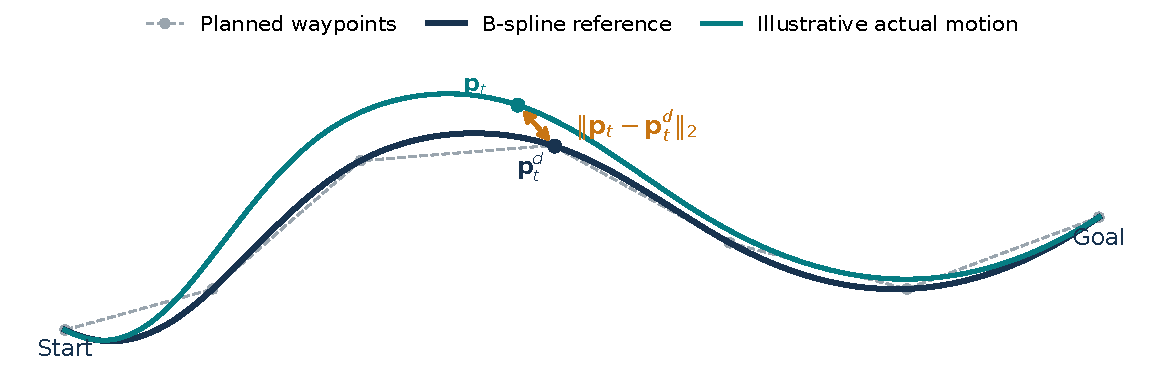
\includegraphics[width=\linewidth]{figures/evaluation_tracking_reference.pdf}
\caption[Smoothed reference and time-matched tracking error]{Conceptual planar view of a three-dimensional tracking task. A B-spline is fitted to planned waypoints; reference samples and actual positions are paired at the same instant. The highlighted separation contributes one term to Equation~\eqref{eq:average_tracking_error}.}
\label{fig:evaluation_tracking}
\end{figure}

A prescribed timing law provides $\bm p_1^d,\ldots,\bm p_T^d$ at the evaluation sampling interval. The reference and its timing are held constant across compared methods.


\clearpage
\section{Curriculum Training}
\label{sec:curriculum_training}

The navigation policy follows a curriculum, progressing from easier tasks toward harder navigation conditions. This lets the policy acquire basic goal-directed behavior before confronting more demanding situations.

The policy has two hidden layers of 64 units. PPO training uses approximately $10^8$ transitions in 4096 parallel environments on an NVIDIA A100, with learning rate $3\times10^{-4}$, discount factor $0.99$ and clipping ratio $0.2$. The environment executes the CBF-corrected command during filtered training, while PPO retains the sampled nominal action.

\begin{figure}[H]
\centering
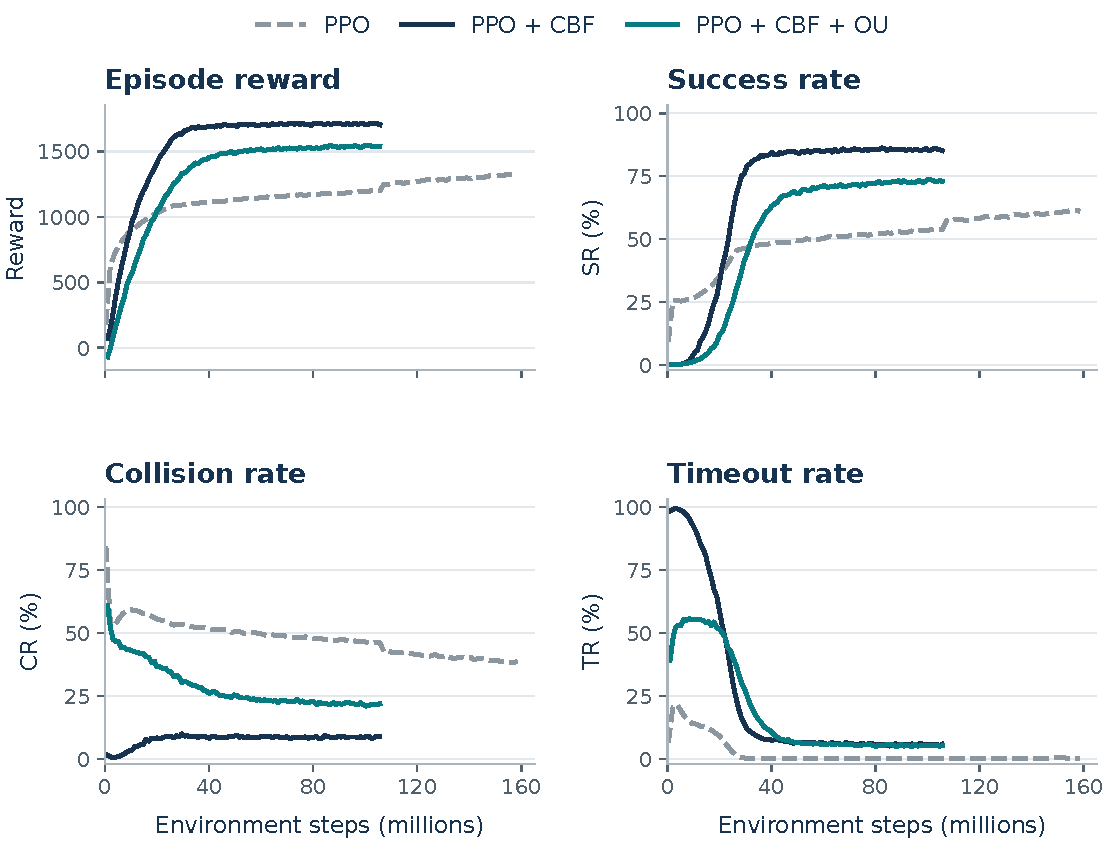
\includegraphics[width=\linewidth]{figures/results_training_curves.pdf}
\caption[Training reward and episode outcomes]{Training reward and episode outcomes for unfiltered PPO, PPO with a CBF filter, and filtered PPO with OU wind. The original plotted values and training horizons are retained. These supplied training histories have no uncertainty bands.}
\label{fig:results_training}
\end{figure}

The no-wind filtered configuration reaches high reward and success earlier in these histories. With OU wind, success rises more gradually and remains lower. The evaluation below holds one policy fixed and changes only the deployed safety filter.

\clearpage
\section{Wind Disturbance Profiles}

Wind is represented through its effect on translational motion. OU profiles retain temporal correlation: successive disturbances fluctuate around a prescribed mean instead of being independent perturbations. The representative profiles in Figure~\ref{fig:results_wind} distinguish drift, stronger sustained disturbance and greater volatility, together with the supplied gust and sinusoidal traces.

\begin{figure}[H]
\centering
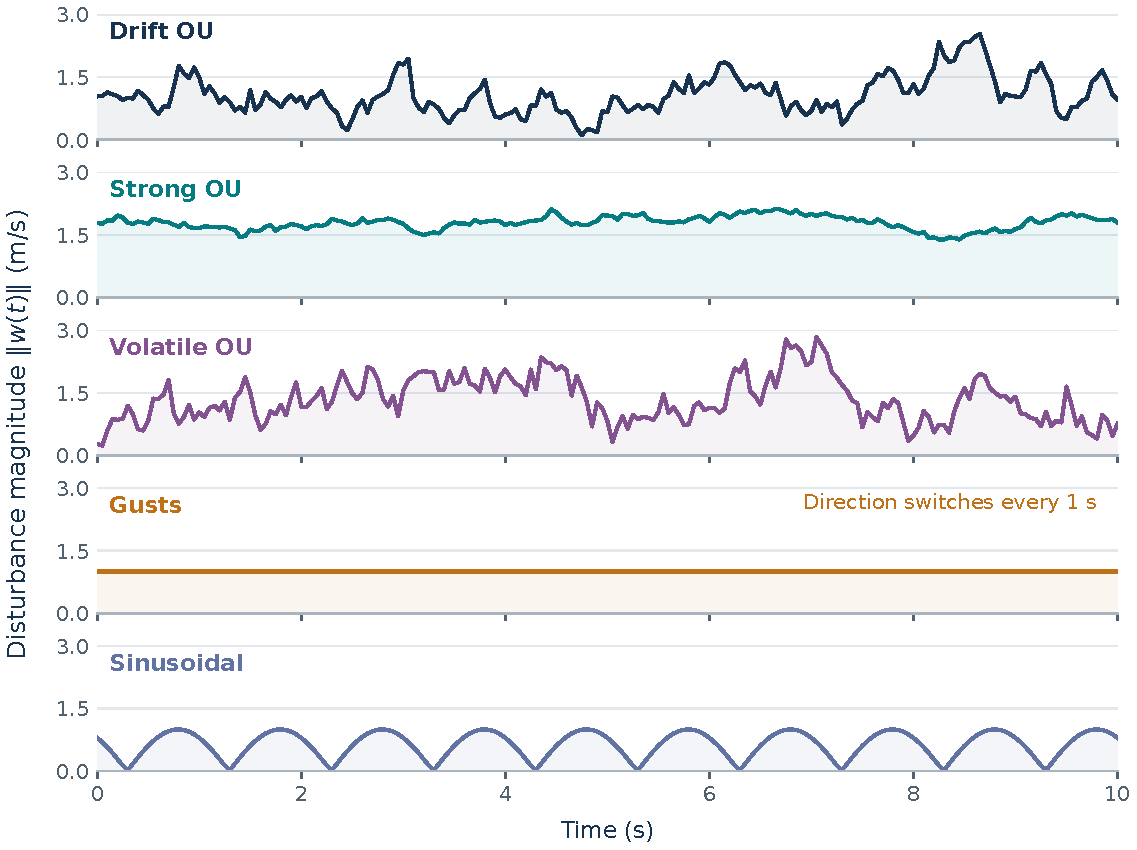
\includegraphics[width=\linewidth]{figures/results_wind_profiles.pdf}
\caption[Representative wind profiles]{Representative disturbance traces with a common magnitude scale. OU denotes Ornstein--Uhlenbeck. The gust profile changes direction every second while retaining a magnitude of 1\,m/s. These are illustrative profiles, not atmospheric measurements.}
\label{fig:results_wind}
\end{figure}

The paired evaluation uses four condition groups: \textbf{calm}, \textbf{steady crosswind}, \textbf{reversing wind} and \textbf{gust-like wind}. Each mission includes one calm condition and five seeded sequences from each noncalm family. These 16 conditions are identical across the compared filters. The five profiles above illustrate temporal behavior; the four benchmark groups define the evaluation split.

\clearpage
\section{Evaluation Protocol}

\subsection{Compared Safety Filters}

All five filters use the same frozen policy: nominal CBF has no disturbance margin; fixed-margin CBF adds 0.50\,m/s; $\mathcal L_1$-style CBF uses disturbance prediction; empirical CVaR-CBF adds the residual tail; and Ours includes the Wasserstein allowance.

For Ours, the observer gain is $0.30I_3$, the residual window contains 64 samples, the tail probability is $\epsilon=0.05$, and $\rho=0.01$\,m/s. The window spans 3.2\,s at the control rate, and the distributional allowance is $\rho/\epsilon=0.20$\,m/s. These settings are fixed before testing. The empirical and Wasserstein variants also have different startup allowances, so their comparison assesses the complete filter configurations.

\subsection{Paired Evaluation and Aggregation}

The comparison retains 79 missions across 20 test environments, giving 1264 episodes per filter. One mission was excluded consistently across all methods and conditions. Paired blocks share the environment, mission and disturbance sequence.

Rates from Equation~\eqref{eq:episode_rates} and continuous quantities are averaged within each environment, then equally across the 20 environments. Standard deviations describe variation between environment means. Paired confidence intervals use 5000 hierarchical bootstrap resamples over environments, missions and conditions.

\clearpage
\section{Evaluation Results}
\label{sec:main_results}
\subsection{Mission Completion and Collisions}

Ours achieves 73.6\% goal success, 17.4\% collisions and 9.0\% timeouts (Table~\ref{tab:results_outcomes}). Its 82.6\% collision-free fraction combines successful episodes and timeouts; SR here counts goal completion only.

\begin{table}[H]
\centering
\caption{Episode outcomes (\%), averaged equally across 20 environments; 1264 episodes per filter. Displayed sums may differ slightly through rounding.}
\label{tab:results_outcomes}
{\small\renewcommand{\arraystretch}{1.3}
\begin{tabularx}{\linewidth}{@{}Yrrr@{}}
\toprule
\textbf{Method} & \textbf{SR $\uparrow$} & \textbf{CR $\downarrow$} & \textbf{TR $\downarrow$}\\
\midrule
Nominal CBF & 62.1 & 37.8 & 0.2 \\
Fixed-margin CBF & 72.3 & 25.3 & 2.3 \\
$\mathcal L_1$-CBF & 70.6 & 27.8 & 1.6 \\
Empirical CVaR-CBF & 73.5 & 19.1 & 7.3 \\
\textbf{Ours} & 73.6 & 17.4 & 9.0 \\
\bottomrule
\end{tabularx}}
\end{table}

Against nominal CBF, Ours improves SR by 11.6 percentage points and reduces CR by 20.4 points. Against empirical CVaR, it has fewer collisions and more timeouts; the SR difference is only 0.1 point, with paired 95\% interval $[-1.64,1.69]$. A goal-completion advantage over empirical CVaR is not resolved.

\subsection{Collision Rates Across Wind Conditions}

\begin{table}[H]
\centering
\caption{Collision rate (\%) by disturbance family, averaged equally across environments: 79 calm episodes and 395 per noncalm family, for each filter.}
\label{tab:results_wind}
{\small\renewcommand{\arraystretch}{1.3}
\begin{tabularx}{\linewidth}{@{}Yrrrr@{}}
\toprule
\textbf{Method} & \textbf{Calm} & \textbf{Steady} & \textbf{Reversing} & \textbf{Gust-like}\\
\midrule
Nominal CBF & 35.4 & 37.2 & 38.7 & 37.9 \\
Fixed-margin CBF & 25.4 & 25.7 & 25.9 & 24.4 \\
$\mathcal L_1$-CBF & 27.9 & 26.1 & 27.0 & 30.4 \\
Empirical CVaR-CBF & 20.4 & 15.8 & 19.4 & 21.9 \\
\textbf{Ours} & 17.9 & 15.5 & 17.3 & 19.2 \\
\bottomrule
\end{tabularx}}
\end{table}

\clearpage
\subsection{Clearance and Reference-Path Deviation}

The archived evaluation reports a geometric reference-path RMSE: at each sample it measures the distance to the closest point on the A* reference, squares these distances, averages them over the episode and takes the square root. This differs from the time-matched average tracking error defined in Section~\ref{sec:tracking_accuracy}. The values below retain their geometric RMSE meaning; the archived aggregates do not provide the timed reference samples needed to calculate the DATT metric.

\begin{table}[H]
\centering
\caption{Minimum clearance and geometric reference-path RMSE, in meters. Entries are equal-environment mean $\pm$ sample standard deviation of environment means.}
\label{tab:results_geometry}
{\small\renewcommand{\arraystretch}{1.4}
\begin{tabularx}{\linewidth}{@{}Ycc@{}}
\toprule
\textbf{Method} & \textbf{Clearance $\uparrow$} & \textbf{Path RMSE $\downarrow$}\\
\midrule
PPO (unfiltered) & $0.166\pm0.129$ & $0.545\pm0.109$ \\
Nominal CBF & $0.178\pm0.124$ & $0.563\pm0.105$ \\
Fixed-margin CBF & $0.200\pm0.115$ & $0.612\pm0.118$ \\
$\mathcal L_1$-CBF & $0.194\pm0.119$ & $0.608\pm0.140$ \\
Empirical CVaR-CBF & $0.215\pm0.110$ & $0.655\pm0.166$ \\
\textbf{Ours} & $0.227\pm0.107$ & $0.673\pm0.184$ \\
\bottomrule
\end{tabularx}}
\end{table}

Ours achieves the largest mean minimum clearance, 0.227\,m, compared with 0.178\,m for the nominal filter. Its path RMSE also increases, from 0.563\,m to 0.673\,m. The filter therefore trades greater deviation from the reference for larger obstacle separation and fewer collisions. The reported clearance is measured outside the evaluation envelope, rather than from the vehicle center.

The unfiltered PPO benchmark has a 44.2\% collision rate and the smallest geometric path RMSE, 0.545\,m. Staying closer to the path does not by itself establish safer navigation. Its matching goal-completion and timeout counts are unavailable in the retained episode archive, so it is not assigned SR or TR values in Table~\ref{tab:results_outcomes}.

Online residual adaptation improves collision avoidance over the nominal filter while preserving the trained policy. Greater clearance comes with more path deviation and timeouts in this static, known-geometry benchmark.

\clearpage
\subsection{Robustness Across Disturbance and Obstacle Density}

Figure~\ref{fig:results_robustness_panels} complements the tables with the disturbance, obstacle-density and safety--tracking comparisons. It retains the collision-free measure, $1-\mathrm{CR}$, so successful episodes and noncolliding timeouts both contribute. This differs from goal-completion SR in Section~\ref{sec:performance_metrics}.

\begin{figure}[H]
\centering
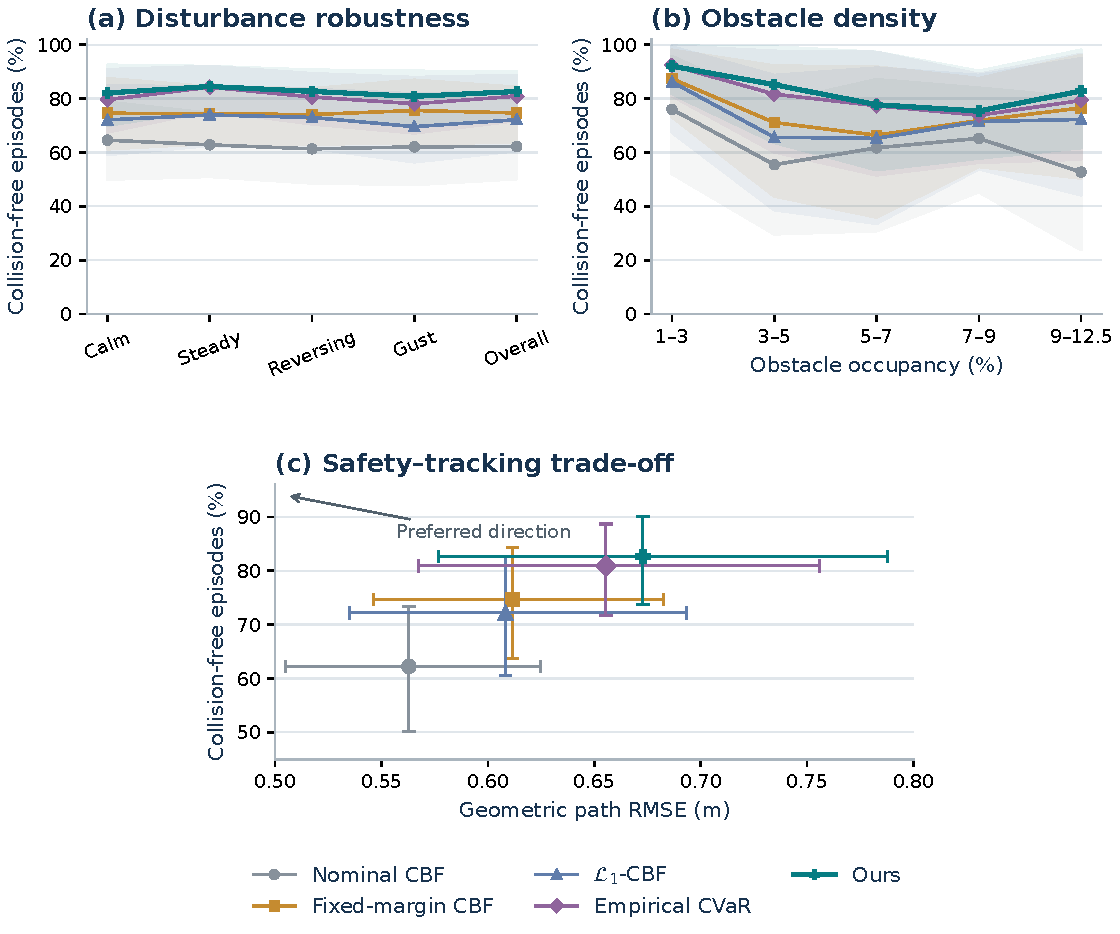
\includegraphics[width=\linewidth]{figures/results_robustness_panels.pdf}
\caption[Disturbance, density and safety--tracking comparisons]{Paired held-out evaluation. (a) Collision-free rate by disturbance. (b) Collision-free rate by obstacle occupancy. (c) Collision-free rate versus geometric path RMSE. Shaded bands and whiskers are hierarchical 95\% bootstrap intervals for one frozen policy; they do not measure variability across policy-training seeds.}
\label{fig:results_robustness_panels}
\end{figure}

The residual-tail filters maintain stronger collision avoidance across disturbance families and occupancy bands. The final panel makes the cost visible: the higher collision-free rate of Ours accompanies greater geometric path deviation. Its interval overlaps that of empirical CVaR, consistent with their close safety results. Appendix~\ref{app:rl_training} summarizes the PPO settings and policy-selection study.

\clearpage
\section{Sim2Sim Evaluation and the Sim2Real Gap}
\label{chap:sim2real}

\subsection{Simulation Performance and Physical Behavior}

A high success rate in simulation does not automatically translate into reliable flight. A policy can exploit its training environment, then struggle with different dynamics on a physical robot. Modeling errors are a central source of this sim2real gap~\cite{litPeng2018}. Imperfect sensing also changes what the robot knows about free space and approaching obstacles~\cite{extnavrl2025}.

The practical extension therefore moves beyond the simplified evaluation environment toward physics-based simulation. Isaac Sim provides rigid-body dynamics, collision models and simulated sensors in a common robotics platform~\cite{extisaacsim}. Its companion framework, Isaac Lab, supports large parallel learning workloads, making this ecosystem useful for both policy development and evaluation~\cite{extisaaclab}.

\begin{figure}[H]
\centering
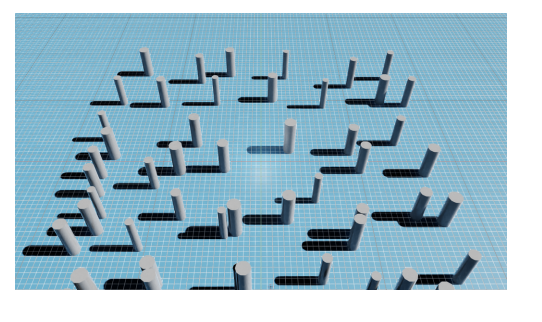
\includegraphics[width=.88\linewidth]{figures/sim2real_arena.png}
\caption[Obstacle arena for the practical navigation extension]{Overview of the obstacle arena used to illustrate the practical navigation extension. Closely spaced pillars create narrow passages and repeated avoidance decisions.}
\label{fig:sim2real_arena}
\end{figure}

This tests whether motion, sensing and collision geometry support the commands selected by the policy.

\clearpage
\subsection{Navigation with Local Perception}

Our sim2sim extension uses Isaac Sim and MuJoCo to examine navigation in richer physical environments. A preplanned A* route is smoothed with a B-spline, providing the reference path. The learned policy follows this reference and reacts when an unforeseen obstacle obstructs it, while the safety layer corrects the proposed command when needed.

The local map is built from simulated LiDAR observations with noise and missing returns, using sensing characteristics inspired by the Livox Mid-360. This changes the navigation problem: the controller must work with the space that has been observed, including gaps in that observation, instead of assuming complete obstacle geometry. The reference path supplies the overall route, and local perception supports the adjustments required during flight.

\begin{figure}[H]
\centering
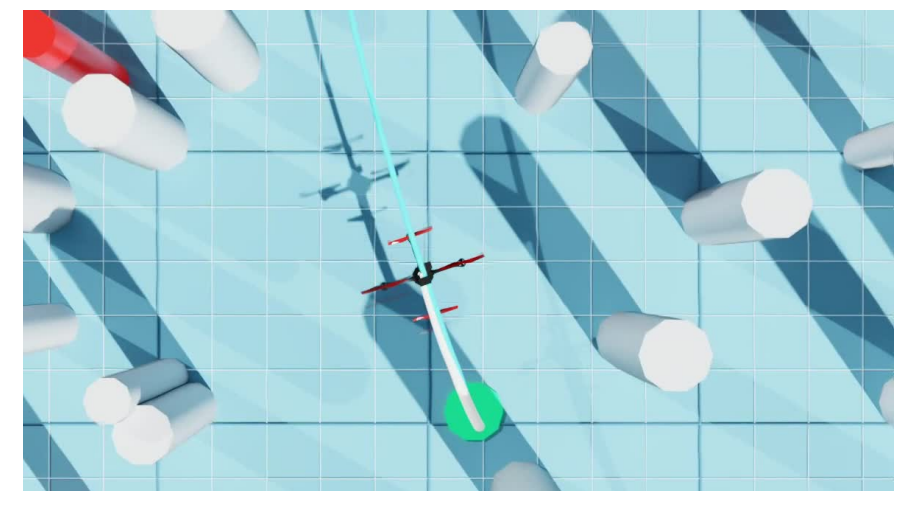
\includegraphics[width=\linewidth]{figures/sim2real_navigation.png}
\caption[Navigation among pillars with a reference path]{Close view of the navigation scene, showing the quadrotor, surrounding pillars, reference path and goal marker. The image illustrates the interaction between route following and local obstacle avoidance.}
\label{fig:sim2real_navigation}
\end{figure}

This stage complements disturbance evaluation by placing the navigation stack in a setting where motion and perception act together. It provides sim2sim evidence toward reducing the sim2real gap; physical flight remains a separate validation step.

\clearpage
\subsection{Comparison with NavRL}

NavRL is a relevant baseline for this setting. It learns UAV navigation with PPO, uses a velocity-obstacle-inspired safety shield and trains many simulated quadrotors in parallel with Isaac Sim. Its authors also demonstrate transfer to physical flight~\cite{extnavrl2025}. This combination of learned navigation, action correction and a physics-based training environment makes it a useful comparison for our practical extension.

Table~\ref{tab:sim2real_navrl} presents our extension benchmark, separately from the known-geometry evaluation in Section~\ref{sec:main_results}. Each scenario contains 72 static obstacles and a different number of dynamic obstacles. The entries compare mission success, collisions and the reported tracking error.

\begin{table}[H]
\centering
\caption[Practical navigation comparison with NavRL]{Practical navigation benchmark. S and D denote static and dynamic obstacles. Higher SR and lower CR and tracking error are preferred; bold values mark the better entry within each scenario.}
\label{tab:sim2real_navrl}
{\small\renewcommand{\arraystretch}{1.45}
\setlength{\tabcolsep}{5pt}
\begin{tabularx}{\linewidth}{@{}lYrrc@{}}
\toprule
\textbf{Scenario} & \textbf{Method} & \textbf{SR (\%)} & \textbf{CR (\%)} & \shortstack{\textbf{Tracking}\\\textbf{error (m)}}\\
\midrule
\multirow{2}{*}{72S + 12D} & Ours & \textbf{99.5} & \textbf{0.5} & \textbf{0.47}\\
 & NavRL & 74.1 & 15.4 & 1.23\\
\midrule
\multirow{2}{*}{72S + 20D} & Ours & \textbf{93.1} & \textbf{6.6} & \textbf{0.80}\\
 & NavRL & 61.6 & 35.1 & 1.15\\
\midrule
\multirow{2}{*}{72S + 40D} & Ours & \textbf{32.1} & \textbf{65.6} & 1.63\\
 & NavRL & 23.7 & 76.3 & \textbf{0.94}\\
\bottomrule
\end{tabularx}}
\end{table}

Ours achieves higher SR and lower CR in all three scenarios. With 12 dynamic obstacles, it reaches 99.5\% SR with 0.5\% CR. With 20, the success advantage is 31.5 percentage points and the collision rate is 28.5 points lower than NavRL. Tracking error is also lower in these first two settings.

With 40 dynamic obstacles, both methods deteriorate sharply. Ours retains higher SR and lower CR, but its tracking error is worse: 1.63\,m versus 0.94\,m. Tracking improves only in the first two scenarios. The extension's tracking-error aggregation is unspecified, so these values are not equated with the time-matched metric or geometric RMSE of Section~\ref{sec:main_results}.
